% $Id: template.tex 11 2007-04-03 22:25:53Z jpeltier $

\documentclass{vgtc}                          % final (conference style)
%\documentclass[review]{vgtc}                 % review
%\documentclass[widereview]{vgtc}             % wide-spaced review
%\documentclass[preprint]{vgtc}               % preprint
%\documentclass[electronic]{vgtc}             % electronic version

%% Uncomment one of the lines above depending on where your paper is
%% in the conference process. ``review'' and ``widereview'' are for review
%% submission, ``preprint'' is for pre-publication, and the final version
%% doesn't use a specific qualifier. Further, ``electronic'' includes
%% hyperreferences for more convenient online viewing.

%% Please use one of the ``review'' options in combination with the
%% assigned online id (see below) ONLY if your paper uses a double blind
%% review process. Some conferences, like IEEE Vis and InfoVis, have NOT
%% in the past.

%% Figures should be in CMYK or Grey scale format, otherwise, colour 
%% shifting may occur during the printing process.

%% These few lines make a distinction between latex and pdflatex calls and they
%% bring in essential packages for graphics and font handling.
%% Note that due to the \DeclareGraphicsExtensions{} call it is no longer necessary
%% to provide the the path and extension of a graphics file:
%% \includegraphics{diamondrule} is completely sufficient.
%%
\ifpdf%                                % if we use pdflatex
  \pdfoutput=1\relax                   % create PDFs from pdfLaTeX
  \pdfcompresslevel=9                  % PDF Compression
  \pdfoptionpdfminorversion=7          % create PDF 1.7
  \ExecuteOptions{pdftex}
  \usepackage{graphicx}                % allow us to embed graphics files
  \DeclareGraphicsExtensions{.pdf,.png,.jpg,.jpeg} % for pdflatex we expect .pdf, .png, or .jpg files
  \usepackage{minted}
\else%                                 % else we use pure latex
  \ExecuteOptions{dvips}
  \usepackage{graphicx}                % allow us to embed graphics files
  \DeclareGraphicsExtensions{.eps}     % for pure latex we expect eps files
\fi%

%% it is recomended to use ``\autoref{sec:bla}'' instead of ``Fig.~\ref{sec:bla}''
\graphicspath{{figures/}{pictures/}{images/}{./}} % where to search for the images

\usepackage{amsmath}
\usepackage{microtype}                 % use micro-typography (slightly more compact, better to read)
\PassOptionsToPackage{warn}{textcomp}  % to address font issues with \textrightarrow
\usepackage{textcomp}                  % use better special symbols
\usepackage{mathptmx}                  % use matching math font
\usepackage{times}                     % we use Times as the main font
\renewcommand{\ttdefault}{\rmdefault} % Sets typewriter font to match the Roman (Serif) font
\usepackage[T1]{fontenc}               % Ensures font encoding handles the switch correctly
\usepackage{cite}                      % needed to automatically sort the references
\usepackage{tabu}                      % only used for the table example
\usepackage{booktabs}                  % only used for the table example
\usepackage{minted}
\usepackage[ruled,vlined]{algorithm2e}
\documentclass{article}
\usepackage{listings}
\usepackage{xcolor}

%% We encourage the use of mathptmx for consistent usage of times font
%% throughout the proceedings. However, if you encounter conflicts
%% with other math-related packages, you may want to disable it.


%% If you are submitting a paper to a conference for review with a double
%% blind reviewing process, please replace the value ``0'' below with your
%% OnlineID. Otherwise, you may safely leave it at ``0''.
\onlineid{0}

%% declare the category of your paper, only shown in review mode
\vgtccategory{Research}

%% allow for this line if you want the electronic option to work properly
\vgtcinsertpkg

%% In preprint mode you may define your own headline.
%\preprinttext{To appear in an IEEE VGTC sponsored conference.}

%% Paper title.

\title{5LSL0 Machine Learning for signal processing - assignment 2}

%% This is how authors are specified in the conference style

%% Author and Affiliation (single author).
%%\author{Roy G. Biv\thanks{e-mail: roy.g.biv@aol.com}}
%%\affiliation{\scriptsize Allied Widgets Research}

%% Author and Affiliation (multiple authors with single affiliations).
%%\author{Roy G. Biv\thanks{e-mail: roy.g.biv@aol.com} %
%%\and Ed Grimley\thanks{e-mail:ed.grimley@aol.com} %
%%\and Martha Stewart\thanks{e-mail:martha.stewart@marthastewart.com}}
%%\affiliation{\scriptsize Martha Stewart Enterprises \\ Microsoft Research}

%% Author and Affiliation (multiple authors with multiple affiliations)
\author{Gheorghiu Cristian Stefan\thanks{e-mail: c.gheorghiu1@student.tue.nl}\\ %
        \scriptsize Student number: 2036967}

%% A teaser figure can be included as follows, but is not recommended since
%% the space is now taken up by a full width abstract.
%\teaser{
%  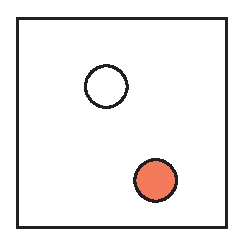
\includegraphics[width=1.5in]{sample.eps}
%  \caption{Lookit! Lookit!}
%}

\usepackage[backend=biber, style=numeric]{biblatex}
\addbibresource{template.bib} % Your .bib file name

%%%%%%%%%%%%%%%%%%%%%%%%%%%%%%%%%%%%%%%%%%%%%%%%%%%%%%%%%%%%%%%%
%%%%%%%%%%%%%%%%%%%%%% START OF THE PAPER %%%%%%%%%%%%%%%%%%%%%%
%%%%%%%%%%%%%%%%%%%%%%%%%%%%%%%%%%%%%%%%%%%%%%%%%%%%%%%%%%%%%%%%%

\begin{document}

%% The ``\maketitle'' command must be the first command after the
%% ``\begin{document}'' command. It prepares and prints the title block.

%% the only exception to this rule is the \firstsection command
\firstsection{Exercise 2.3}
\maketitle
\subsection{2.3.a Requirement}
How do strided downsampling layers in a CNN affect the receptive field?
\subsection{2.3.a Answer}
The growth of receptive field across layers of a CNN based netowrk becomes more and more accelerated as the stride increases. This is particularly demonstrated by the example below, where drawing upon the theoretical receptive field formula \ref{TRFL} we can observe how the aforementioned duality materializes. 

\begin{equation}
TRF_L = 1+\sum_{i=1}^l[(K_i - 1)*\prod_{j=1}^{l-1}]
\label{TRFL}
\end{equation}

   \textbf{For \ref{2} assume a CNN with 2 layers: First layer kernel size is 3x3, stride is 3 and padding is zero. Second layer kernel size is 3x3m stride is 1 and padding is zero}
   
\begin{equation}
\begin{gathered}
TRF_{l=1} = 1 + [(3 - 1) \times 1] = 3 \\
TRF_{l=2} = 1 + [(3 - 1) \times 2] = 4 \\
TRF = TRF_{l=1} + TRF_{l=2} = 7
\label{2}
\end{gathered}
\end{equation}

      \textbf{For \ref{3} assume the same CNN architecture as above but WITHOUT STRIDING.}
   
\begin{equation}
\begin{gathered}
TRF_{l=1} = 1 + [(3 - 1) \times 1] = 3 \\
TRF_{l=2} = 1 + [(3 - 1) \times 1] = 3 \\
TRF = TRF_{l=1} + TRF_{l=2} = 6
\label{3}
\end{gathered}
\end{equation}

%%%%%%%%%%%%%%%%%%%%%%%%%%%%%%%%%%%%%%%%%%%%%%%%%%%%%%%%%%%%%%%%
%%%%%%%%%%%%%%%%%%%%%% START OF ab %%%%%%%%%%%%%%%%%%%%%%
%%%%%%%%%%%%%%%%%%%%%%%%%%%%%%%%%%%%%%%%%%%%%%%%%%%%%%%%%%%%%%%%%
\subsection{2.3.b Requirement}
A CNN without strided downsampling layers is equivariant to the symmetry group of
all integer-pixel translations. If we use two strided downsampling layers in our CNN,
what symmetry group is the network equivariant to? 
\subsection{2.3.b Answer}
As showed in \cite{PhysRevD.104.074504} \cite{cohen2016group} a two strided downsampling CNN layer becomes equivariant to a particular spectrum of translations, primarily constituted from shifts operations as multiples of 2 pixels. More generally, architectures carrying a strider higher than one, can generalize only to lattice sizes that are multiple of the stride combinations. 

\subsection{2.3.c Requirement}
The simulator quantizes the delays to integers, meaning nearby locations will result
in the same simulation results. Create a figure showing which areas result in the
same simulation results for (x, y) source locations (0, 50), (-100, 50), (0, 150) and
(100, 150)cm. Explain your process
\subsection{2.3.c Answer}
The process of determining the areas (e.g., pixel/space coordinates) for which the simulated results (e.g., time delays calculated based on the distance between fixed positions and microphone locations) are considered similar to time delays derived based on distinct coordinates (e.g., space coordinates) is linked to the relative time delays. As Figure \ref{fig:four_mic_array_spqtial_quant} depicts, such zones where discrepancies between the relative time delays do not exist were coloured with green. This space colourisation takes place when the space differences relative to the first microphone are equal to the fixed differences (e.g., (0, 50), (-100, 50), (0, 150) and (100, 150) cm) again to the first microphone. 

The prevalent red colour reflects that sound transmission from the vast majority of space locations will result in arrival delays that are different from what we would usually get if the same signal were forwarded from any of the four known sources. To have this experiment hold true, saving the relative time delays (the difference in arrival time between Mic 1 and the other three mics) is crucial, as I discovered earlier; the absolute travel time changes as you move away.

\begin{figure}[h]
    \centering
    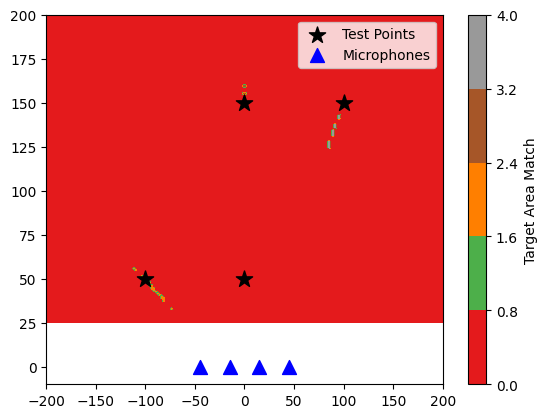
\includegraphics[width=0.9\linewidth]{pictures/time_delays_calculations.png}
    \caption{Spatial Quantization of Relative Time Delays in a Four-Microphone Array}
    \label{fig:four_mic_array_spqtial_quant}
\end{figure}


\subsection{2.3.d Requirement}
Design a 1D neural network with two outputs: the estimated x- and y-coordinate
of the source. Explain your design choices.
\begin{enumerate}
    \item Implement and train your model. Plot both the loss graph and the average
validation accuracy in centimeters over time.
    \item (optional:) You are encouraged to iterate on your design and change things if
you realize your design choices were sub-optimal. Explain the changes you made
to your original design, the reasoning behind those changes, and whether this
resulted in improvement.
\end{enumerate}

\subsection{2.3.d Answer}
\begin{enumerate}
    \item Check both, Figure \ref{fig:loss_1source} and Figure \ref{fig:loss1source_cm}
    \begin{figure}[h]
        \centering
        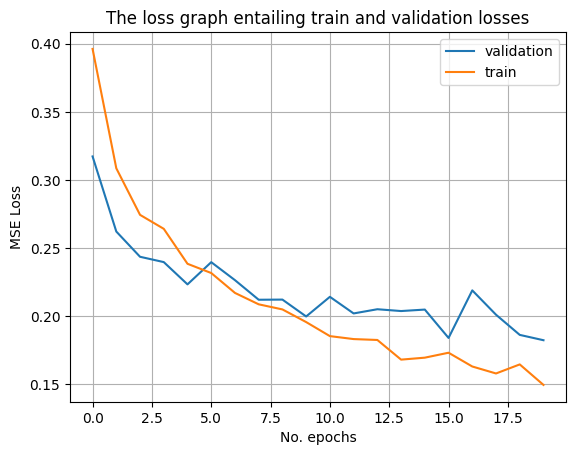
\includegraphics[width=0.8\linewidth]{pictures/loss_graph_2d.png}
        \caption{The loss graph entailing train and validation losses}
        \label{fig:loss_1source}
    \end{figure}
    \begin{figure}
        \centering
        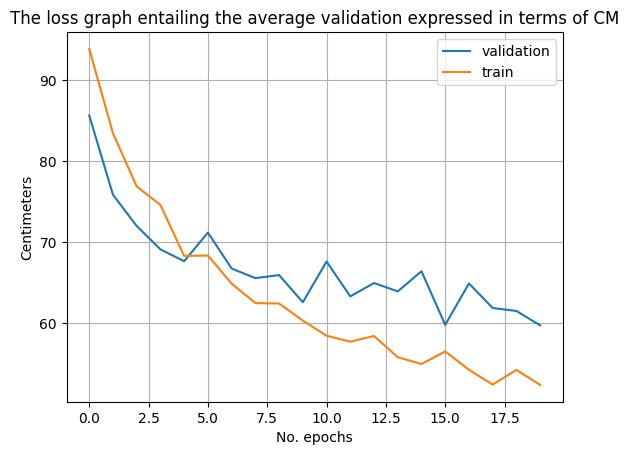
\includegraphics[width=0.9\linewidth]{pictures/loss_1source_cm.png}
        \caption{The loss graph entailing the average validation expressed in terms of CM}
        \label{fig:loss1source_cm}
    \end{figure}
    
    \item A hardly identifiable flaw in the initial architecture not only kept the model performance within an unsatisfactory region (e.g., under 30\% accuracy) but also caused its learning curve to lack any concrete downward trend and to be extremely volatile. I initially suspected the network not to be powerful enough (e.g., ~ to not have enough capacity) and decided to keep on using the same track/.mp3 file to promote overfitting to see whether the model could actually 'learn'. The trial turned out to yield insightful results based on which I counted out the model's architecture from the list of possible culprits. This made me reorient my attention to the custom Dataloader, where I noted by printing out data-related information (e.g., shapes) that the batch dimension remained fixed at 28 (which is the maximum number of training files) irrespective of how large the batch-size variable is. This flaw arose from how I design the magic function  \lstinline|def __len__(self):| to return the length based on the number of training files counted (a maximum of 28).

    
    Such adjustments made for a stable (e.g., lack of spikes/volatility) but not satisfactory convergence, as the model’s performance was far behind the 65\% accuracy bar. This prompted me to explore some feature transformations I could implement and execute during training without accidentally altering any type of information. I came up with \lstinline|AudioPool(nn.Module):|  that encompasses two mean-max pooling operations, meant to retrieve the loudest occurrence/activity over channels and avoid capturing peaks provoked by noisy artifacts.
    
\end{enumerate}
\subsection{2.3.e Requirement}
Calculate the receptive field of your model.
\begin{enumerate}
    \item Verify this result experimentally; explain your process and include a figure.
    \item Does the theoretical result match the receptive field that you find in practice?
\end{enumerate}

\subsection{2.3.e Answer}
\begin{enumerate}
    \item To get up to speed with the class pace, I called in the torchscan module \textcolor{red}{\texttt{summary}} and enabled its argument to true (e.g., \textcolor{red}{\texttt{receptive field=True}}) which adds on the summary table a fifth column encompassing the receptive fields corresponding to each layer in the network. Summing up all the elements, from bottom to top we obtain a \textbf{TRF (theoretical receptive field) of 19}. The prebuilt function has at its core the formula \ref{TRFL}} I used previously. The results can be seen in the Table \ref{tab:model_summary}.

    \item As demonstrated in \cite{araujo2019computing}\cite{bohrium_effective_receptive_field}\cite{luo2016understanding}, but also enforced by the result revealed by my hand-made calculations, the \textbf{TRF as calculated before does not actually match the one I found in practice.} This divergence has its roots deeply buried in the expected/imagined growth of the receptive field (which we assume to be of a linear nature, expanding as more layers L are being added), whereas experiments are showing that the ERF's effective radius (measured by the standard deviation of its Gaussian shape, σ) grows proportionally to the square root of the depth, \sigma \propto \sqrt{L}.

\end{enumerate}

\begin{table}[htbp]
    \centering
    \caption{Model Architecture Summary}
    
    % ---  ---
    \setlength{\tabcolsep}{3pt} % Reduces the horizontal space between columns (default is 6pt)
    \footnotesize               % Reduces the font size of the entire table
    % ---------------------------
    
    \renewcommand{\arraystretch}{1.1}
    \begin{tabular}{llcrr}
        \toprule
        \label{tab:model_summary} 
        \textbf{Layer} & \textbf{Type} & \textbf{Output Shape} & \textbf{Param \#} & \textbf{Receptive Field} \\
        \midrule
        defaultcnn & DefaultCNN & $(-1, 2)$ & 0 & 19 \\
        \quad $\vdash$ n & Sequential & $(-1, 128)$ & 0 & 19 \\
        \quad\quad $\llcorner$ 0 & Conv1d & $(-1, 32, 4800)$ & 256 & 19 \\
        \quad\quad $\llcorner$ 1 & BatchNorm1d & $(-1, 32, 4800)$ & 129 & 13 \\
        \quad\quad $\llcorner$ 2 & LeakyReLU & $(-1, 32, 4800)$ & 0 & 13 \\
        \quad\quad $\llcorner$ 3 & Conv1d & $(-1, 64, 2400)$ & 10,304 & 13 \\
        \quad\quad $\llcorner$ 4 & BatchNorm1d & $(-1, 64, 2400)$ & 257 & 5 \\
        \quad\quad $\llcorner$ 5 & LeakyReLU & $(-1, 64, 2400)$ & 0 & 5 \\
        \quad\quad $\llcorner$ 6 & Conv1d & $(-1, 64, 1200)$ & 20,544 & 5 \\
        \quad\quad $\llcorner$ 7 & BatchNorm1d & $(-1, 64, 1200)$ & 257 & 1 \\
        \quad\quad $\llcorner$ 8 & LeakyReLU & $(-1, 64, 1200)$ & 0 & 1 \\
        \quad\quad $\llcorner$ 9 & AudioPool & $(-1, 128)$ & 0 & 1 \\
        \quad $\vdash$ fc1 & Linear & $(-1, 32)$ & 4,128 & 1 \\
        \quad $\vdash$ activ & LeakyReLU & $(-1, 32)$ & 0 & 1 \\
        \quad $\vdash$ drop1 & Dropout & $(-1, 32)$ & 0 & 1 \\
        \quad $\vdash$ fc2 & Linear & $(-1, 2)$ & 66 & 1 \\
        \midrule
        \multicolumn{5}{l}{\textbf{Trainable params:} 35,618} \\
        \multicolumn{5}{l}{\textbf{Non-trainable params:} 0} \\
        \multicolumn{5}{l}{\textbf{Total params:} 35,618} \\
        \midrule
        \multicolumn{5}{l}{\textbf{Model size (params + buffers):} 0.14 Mb} \\
        \multicolumn{5}{l}{\textbf{Framework \& CUDA overhead:} 0.00 Mb} \\
        \multicolumn{5}{l}{\textbf{Total RAM usage:} 0.14 Mb} \\
        \midrule
        \multicolumn{5}{l}{\textbf{Floating Point Operations on forward:} 105.07 MFLOPs} \\
        \multicolumn{5}{l}{\textbf{Multiply-Accumulations on forward:} 52.15 MMACs} \\
        \multicolumn{5}{l}{\textbf{Direct memory accesses on forward:} 52.18 MDMAs} \\
        \bottomrule
    \end{tabular}
\end{table}



\subsection{2.3.f Requirement}
Once you’re done developing your model with the training and validation set, run
the model on your test set. Explain your process of evaluating the performance and
report your results. Include a representative figure visualizing the performance. Also
comment on how the test-set performance compares to the validation set performance,
and how this compares to the quantization ambiguity found in (c).
\subsection{2.3.f Answer}
To evaluate different architectures and optimize hyperparameters, the model was initially trained on the training set and tuned using the validation set. To put the model's performance evolution in a clearer perspective and demonstrate convergence stability, I then loaded the pre-trained weights and ran the model for 15 epochs over the test set. As shown in Figure \ref{fig:one osurce evolution model}, performance steadily improves during the training-validation phase and remains within the expected optimal threshold (defined by an MSE loss of 0.22 or lower) when evaluated on the test set. \textbf{However, usually the test set is predestinated to one-pass experiment which in this case yielded the following figures: MSE Loss: 0.2237 Test Error in CM: 65.64 cm}.

\begin{figure}[h]
    \centering
    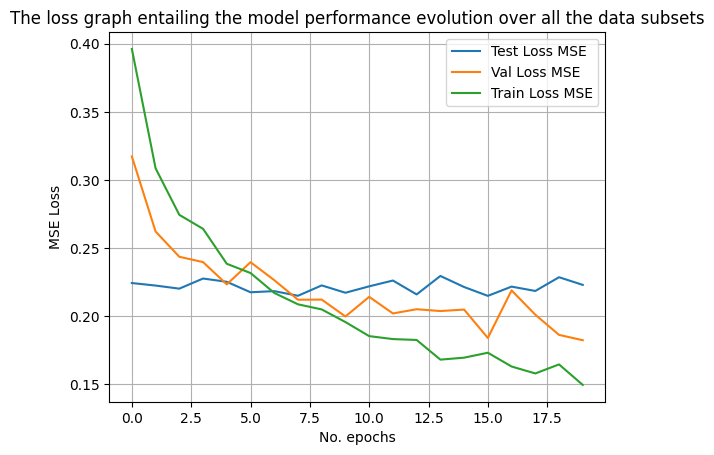
\includegraphics[width=0.9\linewidth]{pictures/overall performance.png}
    \caption{Model performance evolution}
    \label{fig:one osurce evolution model}
\end{figure}

On a slightly different note, the model performance as portrayed by the aforementioned figures is, without a shadow of a doubt, negatively influenced by the quantization ambiguity. If several particular adjustments (such as increasing the bit depth or artificially injecting the noise) were made then we would have attained even a nicer performance than the one shown above. However, for the first part of the assignment, I was more interested in describing the limitation that stems from this kind of quantization ambiguity, which I managed to translate mathematically as shown below in \ref{4}.

\begin{equation}
\begin{gathered}
$T_s = \frac{1}{f_s}$\\
$T_s = \frac{1}{48,000}$\\
$T_s \approx 0.000020833 \text{ seconds}$ (or $20.83 \, \mu\text{s}$)\\
\label{4}
\text{D} = 343 \text{ m/s} \times 0.000020833 \text{ s}=0.0071458meters$\\
\text{D} =0071458m*1000=\textbf{7.1458 mm}
\end{gathered}
\end{equation}
This 7.15 mm value represents the absolute theoretical threshold resolution limit of the adopted sampling rate of 48kHz. If the sound source moves a distance smaller than this limit, the change in the time delay is just to brief to cross into an adjacent digital sample bucket $s_{i-1}$. This sample index that remains unchanged is materialized in identical input tensors making movements less than 7.15 mm "invisible" to the model.

\subsection{2.3.g Requirement}
Design and train a 1D neural network that can locate between 1 and 3 sources
simultaneously. For example, you can use a network where the the coordinates of
the closest source are estimated by the first two outputs, the second source by the
next two, and so forth, with one final network output estimating how many sources
are active. Again, explain your design choices and visualize the training process in a
figure. 
\begin{enumerate}
    \item (optional:) You are encouraged to iterate on your design and change things if
you realize your design choices were sub-optimal. Explain the changes you made
to your original design, the reasoning behind those changes, and whether this
resulted in improvement
\end{enumerate}

\subsection{2.3.g Results}
\begin{enumerate}
    \item The training process can be visualized in the following Figures \ref{fig:mseloss_3sources} and \ref{fig:cmloss_3sources} 

    \begin{figure}[h]
    \centering
    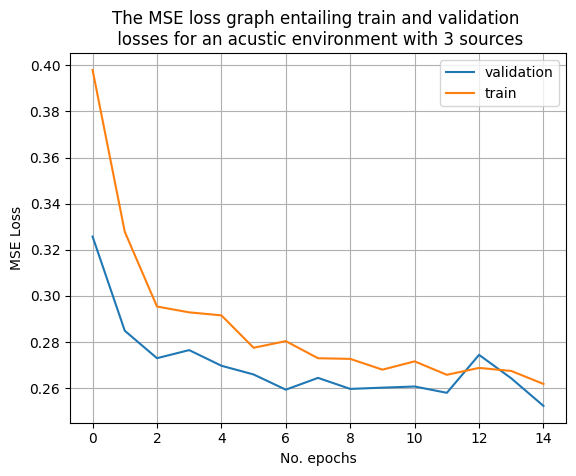
\includegraphics[width=0.8\linewidth]{pictures/The MSE loss graph entailing train and validation losses for an acustic environment with 3 sources.png}
    \caption{Train and Validation losses for an environment with 3 acoustic sources}
    \label{fig:mseloss_3sources}
\end{figure}

\begin{figure}[h]
    \centering
    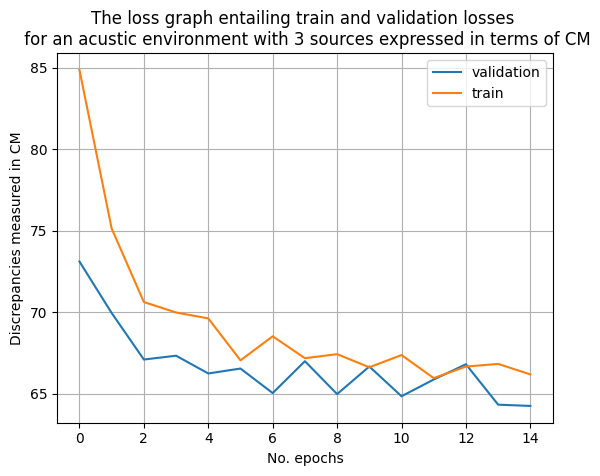
\includegraphics[width=0.8\linewidth]{The loss graph entailing train and validation losses for an acustic environment with 3 sources expressed in terms of CM.png}
    \caption{Train and Validaiton losses expressed in terms of CM for 3 acoustic sources}
    \label{fig:cmloss_3sources}
\end{figure}
    
    \item Laying out through an enumeration the changes I made across multiple sectors, ranging from the network architecture itself to the custom data loader all the way to the training loop in order to accommodate the task at hand:
\begin{enumerate}
    \item Automatic adjustment of the learning rate, commonly known as a learning rate scheduler, using the module named 'ReduceLROnPlateau' equipping 2 patient epochs (patience=5). Reduce the learning rate when a metric has stopped improving.
    \item By setting the argument to None (\lstinline|reduction=None| in the \lstinline|nn.MSELoss()|), the adoption of a dynamic mask becomes possible. Since the network will always generate a fixed number of predictions (e.g., 6 pairs of coordinates) irrespective of how many sources do actually exist, a penalty must be applied only for the existent sources.
    \item Typical adjustments(such as $p=(\text{kernel size}-1)//2$) of CNN hyperparameters (e.g., kernel size, padding and stride) will not make result in rich gains. Starting off with a kernel size that is large enough to capture the maximum delay between the furthest microphone and the source becomes a strictly required adjustment. 
    \item Adopting a sorting rule (e.g. sorting by relative distance between sources and microphones along a single dimension X) that is not restructuring the hierarchical order of the prediction indices turned out to be a game changer as, the model was able to break through the 30\% accuracy plateau much faster than before. On top of that, to provide the network with concise insights regarding to how well it can predict either the pair of coordinates or the number of sources, I created a composite error placing as much weight (95\%) as possible on the coordinates.
\end{enumerate}


\end{enumerate}

\subsection{2.3.h Requirement}
 If we order our outputs by distance from the microphones as suggested above, what
may happen if two sources in a training sample are at similar distances? Is that a
problem, and if so, how could we fix it?

\subsection{2.3.h Answer}
If two sources are at similar distances, slight fluctuations in the model's predictions during training can cause their relative ordering to flip continuously. This is a significant problem because it causes label swapping. The target labels assigned to specific output nodes will suddenly change between training steps. Consequently, at loss computation time, the correspondence between the predictions and the ground truth is destroyed. The loss function will compare a prediction to the wrong source target, yielding massive, unstable penalties that confuse the network and derail the learning curve.
To resolve this, we can abandon fixed heuristic ordering and instead use Permutation Invariant Training (PIT). In PIT, the network computes the loss for all possible permutations of assignments between the predicted outputs and the ground truth targets. It then backpropagates the error using only the permutation that yields the minimum loss, entirely bypassing the need to sort by distance.


\subsection{2.3.i Requirement}
Once you’re done developing your model, run the model on your test set. Ex-
plain your process of evaluating the performance in different scenarios and report your
results. Include representative figures visualizing the performance
\subsection{2.3.i Answer}
The vast majority of adjustments made during the training-validation phase yielded enough of a positive and strong change to make further augmentations or adoptions meaningless. Therefore, based on a known suite of hyperparameters, table \ref{tab:test_results} represents a solid outline of the model performance on unseen data for a varying number of sources. Telling exactly how many acoustic sources the model can handle simultaneously without difficulty (or without having the prediction error deviate from what we’ve seen during training and testing) remains a fairly difficult task given the minor discrepancies we see in the table. As worth trying, the follow-up experiment will consist of increasing the number of sources until the model prediction error completely derails and labeling the breaking point (e.g., 10 sources) as the upper bound of the optimal domain. Furthermore, random assignment of the number of sources might not be an ideal training paradigm. A more favorable and worth applying approach would be to put in place a mechanism that ensures a even exposure of the network to any of the three settings (e.g., 1 , 2  or 3 sources)

\begin{table}[H]
    \centering
    \renewcommand{\arraystretch}{1.2} % Slightly tightened from 1.3 for academic double-column layouts
    \begin{tabular}{@{} c c c @{}} % Removed vertical lines (|) and edge padding (@{})
        \toprule
        \textbf{Number of Sources} & \textbf{Final Test MSE Loss} & \textbf{Final Test Error (cm)} \\
        \midrule
        1 & 0.2633 & 70.43 \\
        2 & 0.2605 & 70.41 \\
        3 & 0.2635 & 71.11 \\
        \bottomrule
    \end{tabular}
    \caption{Final model evaluation on the unseen test set, detailing Mean Squared Error (MSE) and Centimeter (CM) error across varying numbers of active acoustic sources.}
    \label{tab:test_results}
\end{table}


\subsection{2.3.j Requirement}
 Simulate the full recording of both bird sounds in the test set as sources located at
(0, 50)cm and (100, 150)cm respectively. Plot the estimated location error over time
for both. Does the location error correlate with the sound volume of the recordings at
different times? Comment on your findings.

\subsection{2.3.j Answer}
By the book \cite{jekaterynczuk2023sound}, there is often a strong inverse correlation between recording volume (e.g., amplitude) and localization error. When a sound is louder, acoustic sensors (e.g., the four fixed microphones in our case) capture a cleaner, stronger signal, leading to greater accuracy, while low-volume or distorted recordings should result in higher location error. The figure  \ref{fig:placeholder} below partly demonstrates that this statement holds true in practice, though it heavily depends upon how well the model was trained to handle sudden RMS variations. In our case, there is a visible positive correlation between acoustic volume and localization error that, at times, shifts to an inverse correlation. For example, at t = 1.6s, achieving a peak of RMS = 0.22 (which is a medium-height RMS peak for the blue bird), the localization error decreases to a good extent, although this is not sufficient to get a completely accurate prediction. Whereas at t = 8.7s, marked by a double-peak RMS body of RMS = 0.15, the localization error increases by a great extent, clearly marking the positive correlation.

\begin{figure}[h]
    \centering
    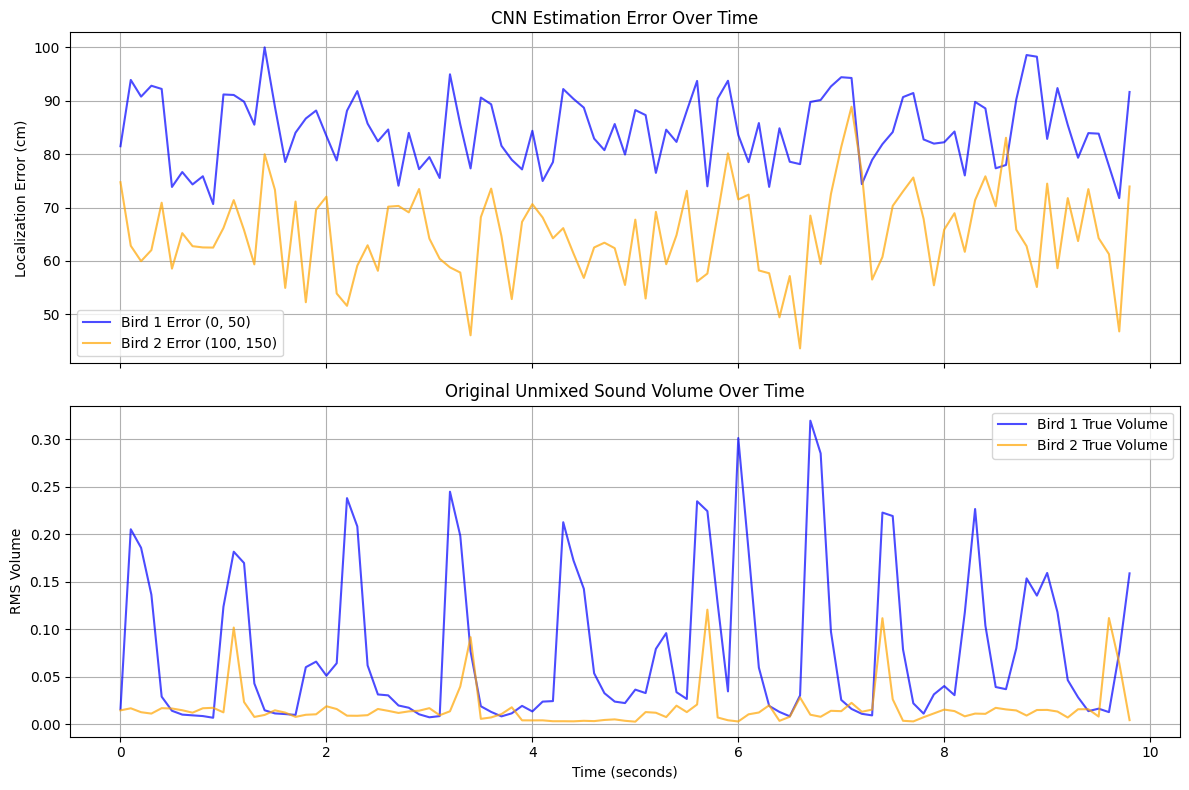
\includegraphics[width=1\linewidth]{Location error correlation with the sound volume.png}
    \caption{Location error correlation with the sound volume}
    \label{fig:placeholder}
\end{figure}
\printbibliography
\end{document}
